\documentclass{article}
\usepackage[american]{babel}
\usepackage[backend=biber,style=nature]{biblatex}
\usepackage[margin=true,inline=true,index=true]{fixme}
\usepackage{grffile}
\usepackage{booktabs}
\usepackage{hyperref}
\usepackage{graphicx}
\usepackage{fullpage}
\usepackage{amsmath}
\usepackage{csquotes}
\usepackage{pdfpages}
\usepackage{placeins}

\renewcommand{\vec}[1]{\mathbf{#1}}


\addbibresource{connectomics motif.bib}
\addbibresource{connectomics motif-relational models.bib}

\DeclareGraphicsRule{.ai}{pdf}{.ai}{}

\title{Automatic discovery of cell types and microcircuitry from neural connectomics}
\author{Eric Jonas$^1$, Konrad Kording$^{2, 3,4}$}

\begin{document}
\maketitle

\begin{small}
\begin{enumerate}
  \item Electrical Engineering and Computer Science, University of California, Berkeley
  \item Department of Physical Medicine and Rehabilitation,
    Northwestern University and Rehabilitation Institute of Chicago,
    Chicago, Illinois
  \item Department of Physiology, Northwestern University, Chicago, Illinois
  \item Department of Applied Mathematics, Northwestern University, Chicago, Illinois
\end{enumerate}
\end{small}

\begin{abstract}
  Neural connectomics has begun producing massive amounts of data,
  necessitating new analysis methods to discover the biological and
  computational structure. It has long been assumed that discovering
  neuron types and their relation to microcircuitry is crucial to
  understanding neural function. Here we developed a nonparametric
  Bayesian technique that identifies neuron types and microcircuitry
  patterns in connectomics data. It combines the information
  traditionally used by biologists in a principled and probabilistically-coherent manner, including  including connectivity, cell body
  location and the spatial distribution of synapses. We show that the
  approach recovers known neuron types in the retina and enables
  predictions of connectivity, better than simpler algorithms. It also
  can reveal interesting structure in the nervous system of
  C. elegans and a historic microprocessor.
  Our approach extracts structural meaning from
  connectomics, enabling new approaches of automatically deriving
  anatomical insights from these emerging datasets.
\end{abstract}

\listoffixmes

\section*{Introduction}
Emerging connectomics techniques \autocite{Morgan2013,Zador2012}
promise to quantify the location and connectivity of each neuron
within a tissue volume. These massive datasets will far exceed the
capacity of neuroanatomists to manually trace small circuits, thus
necessitating computational, quantitative, and automatic methods for
understanding neural circuit structure.  The impact of this kind of
high-throughput transition has been seen before -- the rise of sequencing
techniques necessitated the development of novel computational methods
to understand genomic structure, ushering in bioinformatics as an
independent discipline \autocite{Koboldt2013}. 

The brain consists of multiple kinds of neurons, each of which is
hypothesized to have a specific role in the overall
computation. Neuron types differ in many ways, e.g. chemical or
morphological, but they also differ in the way they connect to one
another \autocite{Seung2014}. In fact, the idea of well defined,
type-dependent local connectivity patterns (microcircuits) has a long
history \autocite{Passingham2002}, and is prominent in many areas,
from sensory (e.g. retina, \autocite{Masland2001} to processing
(e.g. neocortex \autocite{Mountcastle1997}) to movement (e.g. spinal
cord) \autocite{Grillner2005}.  These sorts of repeated computing
patterns are a common feature of computing systems, even arising in
human-made computing circuits. It remains an important challenge to
develop algorithms to use connectivity-based anatomical data
(connectomics), to automatically back out underlying microcircuitry.
already begun, focusing on

The discovery of structure is a crucial aspect of network
science. Early approaches focused on global graph properties, such as
the types of scaling present in the network \autocite
{WattsStrogatz1998}.  While this approach leads to an understanding
of the global network, more recent work aims at identifying very small-scale
repeat patterns, or “motifs” in networks\autocite{Milo2002}. These motifs
are defined not between different node types, but rather represent repeated
patterns of topology. 

The discovery of structure in probabilistic graphs is a well-known
problem in machine learning. Commonly used algorithms include
community-based-detection methods \autocite{Girvan2002}, and
stochastic block models \autocite{Nowicki2001}.  While these
approaches can incorporate the probabilistic nature of neural
connections \autocite{Hill2012} they do not incorporate the additional
richer structure present in connectomics data -- the location of cell
bodies, the spatial distribution of synapses, and the distances
between neurons. Of particular importance is that the probability of
connections has a strong spatial component, a factor that is hard to
reconcile with many other methods. A model attempting to fully capture
the variation in the nervous system should take into account the broad
set of available features.

When it comes to neuroscience and other computing systems, we expect
patterns of connectivity much more complex than traditional motifs
exhibiting a strong spatial dependence arising from the complex
genetic, chemical, and activity-based neural development processes.

To address these challenges, here we describe a Bayesian non-parametric
model that can discover circuit structure automatically from
connectomics data: the cell types, their spatial patterns of
interconnection, and the locations of somata and synapses. We show
that by incorporating this additional information, our model both
accurately predicts the connection as well as agrees with human
neuroanatomists as to the identification of cell types. We take as
inspiration previous work on identifying cell types automatically from
morphology \autocite{Guerra2011} and electrophysiology
\autocite{Druckmann2013}. 

We primarily focus on the recently-released mouse retina connectome
\autocite{Helmstaedter2013}, but additionally examine the \textit{C. elegans}
connectome \autocite{White1986}.  Comparing the cell types discovered
by the algorithms with those obtained manually by human anatomists
reveals a high degree of agreement. We thus present a scalable
probabilistic approach to infer microcircuitry from connectomics data
available today and in the future.

\begin{figure}
  \centering 
  \centerline{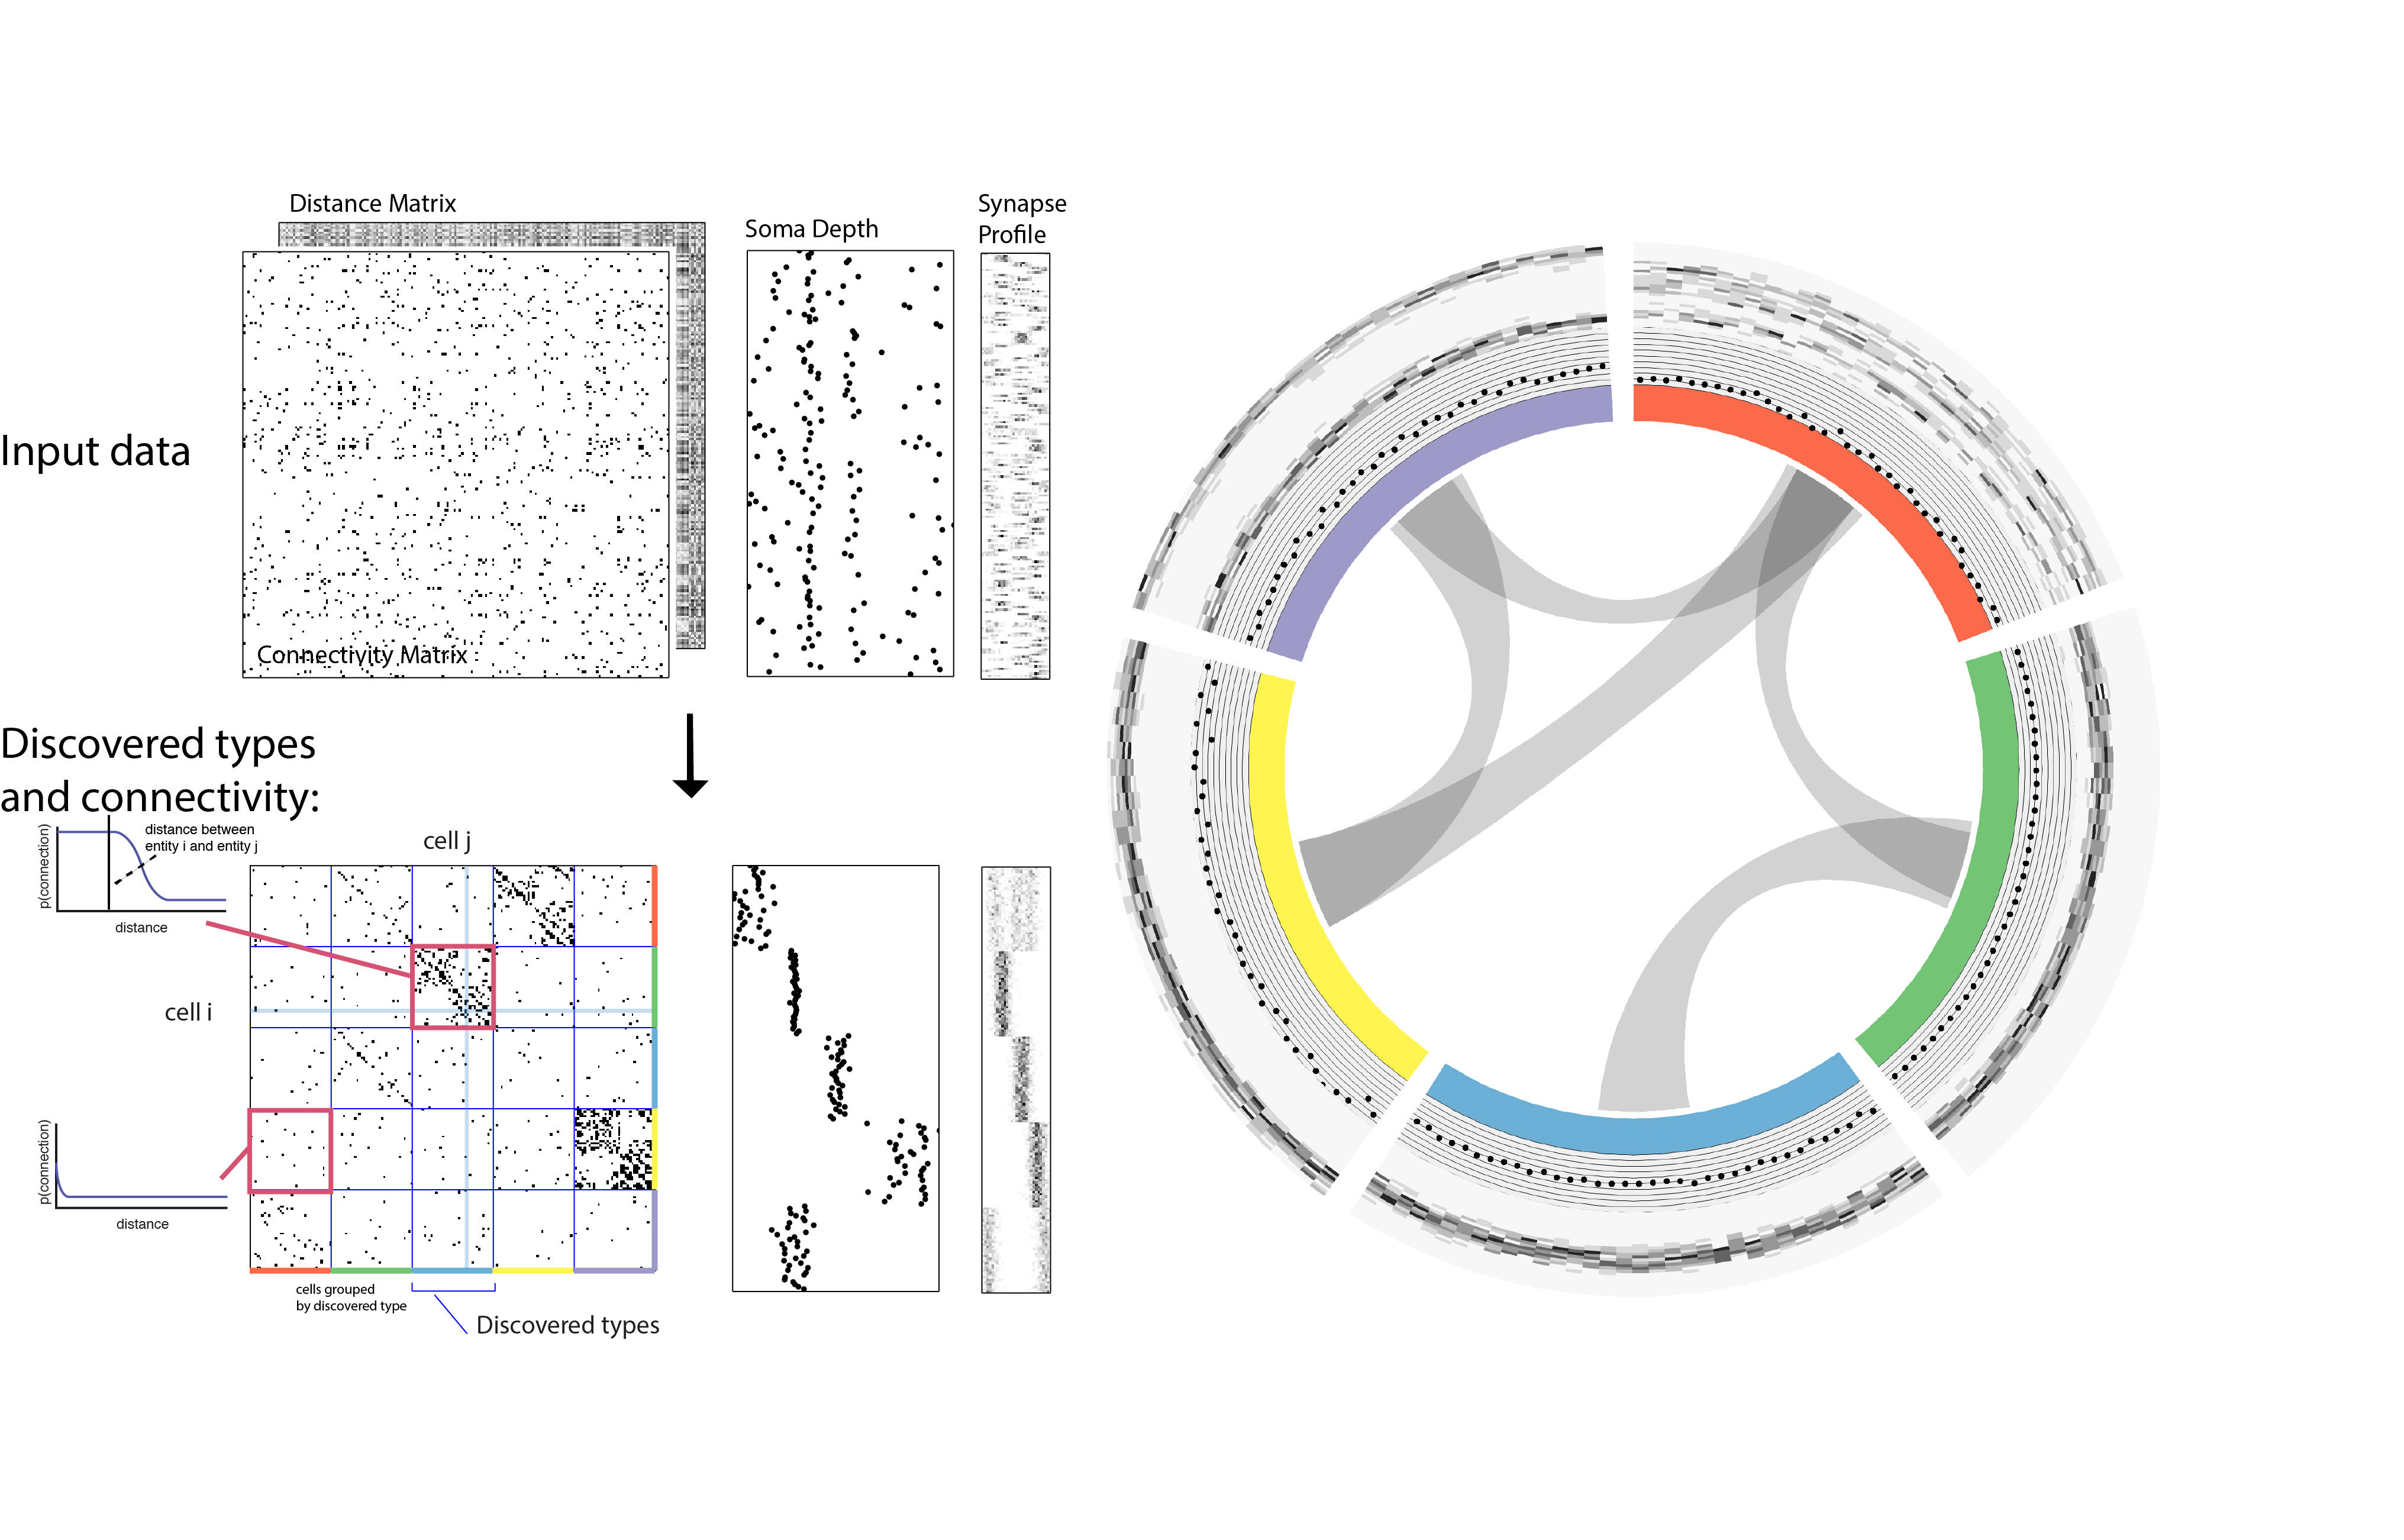
\includegraphics[width=110mm]{fig1b.ai}}
  \caption{Deriving circuitry and cell types from connectomics data
    a. As input we take the connectivity between cells (b), the
    distance between them (c), the depth of the cell bodies (d), and
    the depth profile of the synapses (e). f. Our algorithm discovers
    hidden cell types in this connectivity data by assuming all cells
    of a type share a distance-dependent connectivity profile, similar
    depth, and a similar synaptic density profile, with cells of other
    types.  This results in a clustering of the cells by those hidden
    types. f.) shows the cell connectivity matrix with cells of the
    same type grouped together. g.) shows the learned probability of
    connection between our different types at various distances -- in
    this case, the cells are likely to connect when they are
    close. h. shows the probability of connection between two cell
    types that very rarely connect -- there's a background ``base''
    connection rate to account for errors in data, but the probability
    is very low.  i.) shows that we also recover the expected
    laminarity of types and the depth-specific synaptic
    connectivity. j.) We then plot how the connectivity between these
    types changes as a function of distance between the cell bodies to
    better understand short-range and long-range connectivity
    patterns. }


\label{fig:overview}
\end{figure}

\section*{Methods}


We build a structured probabilistic model which begins with the
generic notion of a cell being a member of a single type -- and these
types affect soma depth, distribution of synapses, as well as a cell
type and distance dependent connection probability. For example,
retinal ganglion cells may synapse on nearby, but not far away,
amacrine cells, with bipolar cells clearly tesselating space and
synapsing on both. In machine learning parlance, our method is
“unsupervised” -- it seeks to discover structure in data and make
predictions in the absence of training data. Rather than taking in
examples of types annotated by human neuroanatomists, we instead start
with the weakest possible assumption in an attempt to algorithmically
discover this structure. We contrast this with the supervised
approaches taken in \autocite{Guerra2011}, where there is high
confidence in the (morphologically-defined) types and then a
supervised classifier is built, as our goal here is explicitly
discovery of types.

\begin{figure}
  \centering 
  \centerline{\includegraphics{synthetic.ai}}
  \caption{Correct recovery of true numbers of hidden types in
    synthetic data when incorporating spatial information. a.) The
    infinite stochastic block model (which only uses connectivity
    information) over-estimates the number of classes as it fails to
    take distance into account, whereas our modeling of the
    combination of distance and connectivity finds close to the true
    number of classes. b.) ARI, a measure of ``correct clustering'',
    for different true class counts, between our model and a
    traditional iSBM. c.) For synthetic data, type discovery based
    only on connectivity are tiny spatially-localized groups -- in
    contrast, our model recovers the true spatial extent of the
    underlying types.  }
\label{fig:synthetic}
\end{figure}

From these assumptions (priors) we develop a generative Bayesian model
that estimates the underlying cell types and how they connect. We take
as input (fig ~\ref{fig:overview}a) the connectivity matrix of cells
(fig ~\ref{fig:overview}b) , a matrix of the distance between cells
(fig ~\ref{fig:overview}c), the per-cell soma depth (fig
~\ref{fig:overview}d) and the depth profile of the cell's synapses
(fig ~\ref{fig:overview}e). We perform joint probabilistic inference
to automatically learn the number of cell types, which cells belong to
which type, their type-specific connectivity, and how connections
between types vary with distance. We also simultaneously learn the
soma depth associated with each type and the typical synaptic density
profile (fig ~\ref{fig:overview}f-h.).

We start with a model for connectivity, the infinite stochastic block
model (iSBM)\autocite{Kemp2006a,Xu2006}, which has been shown to
meaningfully cluster connection graphs while learning the number of
hidden groups, or types. We extend this approach by adding distance
dependence to model salient aspects of microcircuitry via logistic and
exponential distance-link functions.  We form a unimodial model of cell
body depth and a multimodal synapse density profile model (see
Methods for mathematical details).

As an illustrative example, consider a network with only three cell
types, labeled A, B, and C. Assume these cells are uniformly
distributed in space, and that the probability of connection between
any two cells, $c_i$ and $c_j$, depends only on their type and their
distance, according to a logistic (sigmoidal) function. Let A connect
only to nearby B and C cells, but B connect to any C regardless of
distance. This is the prior intuition our model is designed to capture. 


For the basic link-distance model, we take as input a connectivity
matrix $R$ defining the connections between cell $e_i$ and $e_j$, as
well as a distance function $d(e_i, e_j)$ representing a (physical)
distance between adjacent cells.  See
the supplemental material for extension to multiple connectivity
matrices. We assume there exist an unknown number $K$ of latent
(unobserved) cell types, $k \in \{1, 2, 3, \dots, K\}$, and that each
cell $e_i$ belongs to a single cell type. We indicate a cell $e_i$ is
of type $k$ using the assignment vector $\vec(c)$, so $c_i = k$. The
observed connectivity between two cells $R(e_i, e_j)$ then depends
only on their latent type and their distance through a link function
$f(\cdot, d(e_i, e_j))$. We assume $f$ is parameterized based on the
latent type, $c_i=m$ and $c_j=n$, via a parameter $\eta_{mn}$, as well
as a set of global hyper parameters $\theta$, such that the link
function is $f(d(e_i, e_j) | \eta_{mn}, \theta)$.

We then jointly infer the posterior distribution of the
class assignment vector $\vec(c) = \{c_i\}$, the parameter matrix
$\eta_{mn}$, and the global model hyperparameters $\theta$ :

\begin{equation}
  p(\vec{c}, \eta, \theta | R ) \propto \prod_{i, j} p(R(e_i, e_j) | f(d(e_i, e_j) | \eta_{c_ic_j}), \theta) \prod_{m, n} p(\eta_{mn} | \theta)  p(\theta) p(\vec{c} | \alpha) p(\alpha) p(\theta)
\end{equation}

In our subsequent analysis makes use of both the full posterior
distribution over these parameters as well as the most probable, or
maximum \textit{a posteriori} (MAP), estimate.


For the retina data, we then extend the model with the additional
features indicated. Cell soma depth is modeled as a
cell-type-dependent Gaussian distribution with latent (unknown)
per-type mean and variance. Similarly, each cell has some number $N_i$
of synapses, each of which is drawn from a cell-type-specific density
profile with up to three modes.

Inference is performed via Markov-chain Monte Carlo (MCMC) via three
composable transition kernels -- one for structural, one for per-type
parameters, and one kernel for global parameters and
hyperparameters. Details of data preprocessing, inference parameters,
and runtime can be found in the Supplementary Methods section.


\subsection*{Metrics}
To evaluate the quality of the model fit, we need to use information
that quantifies aspects of the data for which we have ground truth
information. We focus on two aspects of performance. First, if the
model works well, then the probability that a pair of neurons is of
the same type should be high if the neurons actually are of the same
type. Second, the model should assign a high probability of connection
between two cells if they have a connection in the underlying data. We
term these two factors clustering accuracy and link prediction
accuracy.

To assess the accuracy of a clustering compared to that determined by
neuroanatomists, we employ three metrics -- clustering homogeneity,
clustering completness, and the adjusted Rand Index. All metrics equal
1.0 when two clusterings completely agree. Homogeneity reflects the
degree to which a found cluster or type contains only a single true
type. Completeness measures how much of a true type is contained
within a single identified type -- a completeness of 1.0 means no true
type is split into multiple subtypes. ARI is a metric that reflects both measures (See
supplemental for more information). 

To assess the accuracy of the model for connections, we use link
prediction accuracy. If our model accurately captures the true
structure of the data, it should be good at predicting if a link
exists.  We thus train the model on the data with a subset of the
links marked as unobserved and thus compute our predictive
accuracy. We perform 10-way cross validation on a given dataset \autocite{Guerra2011}, learn
the resulting model, and use that model to predict the missing
synapses. Each potential link between cells is assigned a probability,
and we compute the area under the curve (AUC) for the resulting ROC
curve. An AUC of 1.0 means that we perfectly predict the presence and
absence of the missing synapses. We use link prediction accuracy to
quantify how good the model is at discovering the underlying
connectivity.  


\section*{Results}
We will first establish that our algorithm works properly and try to
understand its properties using simulated data. Subsequently we will
analyze in detail a dataset on the retina. Lastly we will briefly
discuss the analysis of data from the worm \textit{c.elegans} and from
an ancient microprocessor.


\subsection*{Validation with simulated data where ground truth is known}
To validate our model, we performed a series of simulations to test if
the model can accurately recover the true underlying network structure
and cell type identity.  We thus simulate data for which we know the
correct structure and compare the estimated structure based on the
algorithm (see methods) with the one we used for simulation. We find
that the model does a good job of recovering the correct number of
cell types, (fig~\ref{fig:synthetic}a), the the cell identities
(fig~\ref{fig:synthetic}b), and the spatial extent of each type
(fig~\ref{fig:synthetic}c).  For comparison, we show the results from
instead using the infinite stochastic block model
(fig~\ref{fig:synthetic}a, b, c, black line) which assumes that only
cell type matters, and thus finds small neighborhoods of connected
nodes (instead of global connectivity patterns). This contrast shows
that while the regular block model can not correctly deal with
distance dependent connectivity, our model can. Our model converges
relatively quickly (see supplemental) to an estimate of the most
probable values for the cell types, which is enabled by using a
combination of simulated annealing and parallelized Markov chain Monte
Carlo (see methods for details). Thus our model at least is promising
to be applied to biological datasets.



\subsection*{Model Mismatch}
We next analyze how our model performs in cases where the data are
generated with assumptions different from ours.  To understand the
properties of our model, we attempt connectivity inference on four
sets of synthetic data. This helps us understand what our model would
do if the data does not obey our assumptions.

We thus generate ten sets of synthetic data from each of four existing
models.  The distance-dependent stochastic block model assumes type
depends on distance, the traditional stochastic block model has no
notion of distance, the mixed membership block model assumes type is
combinatorial, and the latent position cluster model assumes that type
is clustered-but-continuous.

If the data is sampled from our model, inference according to our
model, unsurprisingly, is good by all measures. It correctly estimates
the number of cell types; it is good at predicting connectivity (high
AUC); it agrees with human classification (Rand index); it discovers
all types, and leads to homogeneous estimates
(Fig. \ref{fig:othermodel} first row). If the data comes from a block
model without distance dependence, we see that it still does well on
all meaningful measures (Fig. \ref{fig:othermodel} second row). This
is unsurprising, as our model learns the distance dependence, even its
absence. For the mixed membership model (Fig. \ref{fig:othermodel}
third row), the model grossly overestimates the number of types, by
basically allocating a type for each combination of
memberships. Otherwise it still performs relatively well. Lastly, for
the latent position clustering model (Fig. \ref{fig:othermodel} fourth
row), the model does poorly. If type is continuous instead of discrete
then our model is basically trying to cover a continuous set with a
discrete scenario leading to rather poor performance. However, as we
do expect cell types to have a discrete biological basis we might
expect our model to do well with real data.


\begin{figure}
  \centering 

  \includegraphics[width=6.0in]{synthdifferent.ai}
  \caption{Model inferences when true generating model differs from
    our distance-block-model prior. Horizontal columns show results
    with synthetic data generated according to the latent position
    cluster model, the mixed membership block model, the non-distance
    dependent stochastic block model, and the distance dependent
    stochastic block model. In all cases histograms represent
    posterior distribution over indicated metric. a.) The number of
    types found by the model, vertical dash line indicates ``true''
    type number (not applicable to mixed membership model). b.) The
    area under the ROC curve, indicating link prediction accuracy. c,
    d, e.) Clustering metrics quantifying degree of type agreement
    with known ground truth. }

  \label{fig:othermodel}
\end{figure}



\subsection*{Sensitivity to Edge Effects} 

\begin{figure}
  \centering 
  \centerline{\includegraphics[width=3.5in]{edgeeffects.pdf}}
  \caption{We generate two sets of synethetic data, one with
    spatially-dependent connectivity and one without. We measure the
    variance in the connectivity-distance plot for randomly selected
    regions of each dataset, ranging from single-cells to the entire
    volume. We see that while selecting too small of a region can 
    destroy the appearance of distance-dependent connectivity, 
    it does not create it in non-spatial data}
\label{fig:edgeeffects}
\end{figure}

Connectomic efforts so far have reconstructed only small sections of
neural tissue. Consequently, many connections to cells outside that tissue
volume will be lost. We are concerned that this selective elimination
of connectivity along the boundary might give the appearance of
distance-dependent connectivity when there is none. We thus performed
simulations to check if edge effects could destroy spatial structure
and if edge effects could introduce artificial, spurious spatial
structure. We measure the degree to which distance-dependent effects
can arise from selecting regions that are smaller than the ``scale''
of connectivity (fig ~\ref{fig:edgeeffects}). We do this by generating
two collections of synthetic datasets -- one with distance-dependent
connectivity and one without.  We then in each dataset randomly
examine contiguous circular regions with area varying from zero to the
entire volume, and empirically calculate the spatial variance in
type-dependent connectivity.  We find that, if there is no
distance-dependence, edge effects do not artificially introduce
distance dependence. However, if the section we are examining is too
small, our model can miss the distance dependence. Thus with respect
to distance-dependent connectivity inference, our model errs on the
side of caution. But we also find that for spatial extend that is
similar to the currently available datasets the effects of this are
quite limited.

\subsubsection*{Learning types and circuitry in the retina}

\begin{figure}
  \centering 
  \centerline{\includegraphics[width=160mm]{mouseretina2.ai}}
  \caption{Discovering cell classes in the mouse retina connectome. Here
we show the maximum a posteriori (MAP) estimate for the types in the mouse
retina data. 
    a.) Input connectivity data for 950 cells for which soma positions
    were known. b. clustered connectivity matrix, each arbitrary color
    corresponds to a single type, and will be used to identify that type in the remainder
    of the plot. c.)  The spatial distribution of our cell types
    -- each cell type tessellates space. Colors correspond to those in b.)
    d.) Connectivity between our clusters as a function
    of distance -- the cluster consisting primarily of retinal
    ganglion cells (brown node on graph) exhibits the expected near and
    far connectivity.}
\label{fig:mouseretina}
\end{figure}

The mouse retina \autocite{Masland2001} is a neural circuit which we
expect to have connectivity patterns that are well approximated by our
generative model. It is known that there are multiple classes of cells
that can be broadly grouped into: ganglion cells that transmit
information to the rest of the brain, bipolar cells that connect
between different cells, and amacrine cells that feed into the
ganglion cells. Recent research \autocite{Helmstaedter2013} has
produced a large dataset containing both the types of cells from
orthogonal approaches, and also the connectivity matrix between all
reconstructed cells.

The algorithm took less than 4 hours to perform inference, dividing
neurons into a set of cell types (fig~\ref{fig:mouseretina}c, each
wedge is a type). For each pair of neurons there is a specific
distance dependent connection probability
(fig~\ref{fig:mouseretina}b,c,d), which is well approximated by the
model fit. Moreover, each type of cell is rather isotropically
distributed across space (fig~\ref{fig:mouseretina}e) as should be
expected for true cell types.

Comparing the results of the algorithm to other information sources
allows evaluating the quality of the type determination. Our types
closely reflect the (anatomist-determined) segmentation of cells into
retinal ganglion, narrow amacrine, medium/wide amacrine, and bipolar
cells (fig~\ref{fig:mouseretina}c, outermost ring). We find that the
types we find tend to reflect the known laminar distribution in the
retina (fig~\ref{fig:mouseretina}c, middle ring). 

The algorithm yields a separation of neurons into a smaller number of
types than the fully granular listing of 71 types found by the
original authors of the paper, although is still highly correlated
with those finer type distinctions (see
supp~\ref{supp:mouseretina}. It is our expectation that, with larger
datasets, even closer agreement would be found.

Our fully Bayesian model produces a distribution over probable
clusterings.  Figure~\ref{fig:mouseretina_compare} shows this
posterior distribution as a cell-cell coassignment matrix, sorted to
find maximum block structure. Each large, dark block represents a
collection of cells believed with strong probability to be of the same
type. When we plot (fig~\ref{fig:mouseretina_compare}b) the
anatomist-derived cell types along the left, we can see that each
block consists of a roughly-homogeneous collection of types. 

We evaluate our model along three sets of parameters
(Fig.\ref{fig:mouseretina_compare}): how closely does our clustering agree
with neuroanatomists' knowledge?  Given two cells, how accurately can
our model predict the link between them? And how closely does the
spatial extent (within a layer) of our identified types agree with the
known neuroanatomists.

For our model we show the receiver opererating characteristic curve
(ROC curve) (fig~\ref{fig:mouseretina_compare}d) whcih shows how the
true and false positive rates trade off. We plot the posterior
distribution of the area under this curve in
figure~\ref{fig:mouseretina_compare}e. We then plot the 
posterior distribution for cluster agreement metrics -- completeness,
homogeneity, and ari (figure~\ref{fig:mouseretina_compare}f). We see
that our model tends to over-cluster -- some of the finest-granularity of
neuroanatomist types are grouped as a single type by our model. 

We compare link prediction accuracy across the
methods, including our own (Fig.\ref{fig:mouseretina_compare}g AUC, red).  We find that
given the dataset many techniques allow for good link-predictive
accuracy. All the methods allow decent link prediction with an AUC in
the 0.9 range. However, our algorithm clearly outperforms the simple
statistical models that only use connectivity.

As a second measure we compare link prediction accuracy across the
methods (Fig.\ref{fig:mouseretina_compare}g ARI, blue). We find that our
algorithm far outperforms the controls. We also find that when it is
based on more of the same information used by anatomists use then it
gets better at agreeing with these anatomists. In particular, using
connectivity, distance, synapse distribution and soma depth leads to
the highest ARI. When using the available information the algorithm
produces a good fit to human anatomist judgments.

Finally we look at the spatial extent of the discovered types both
within a layer and between layers (Fig.\ref{fig:mouseretina_compare}
h). We see that, in the absence of distance information, mere
connectivity information results in types which only span a small
region of space -- essentially “local cliques”. Incorporation of
distance information results in types which span the entire extent of
the layer. The depth variance of all models continues to be
substantially larger than that predicted by human anatomists -- future
directions of work include attempting to more strongly encode this
prior belief of laminarity.


\begin{figure}
  \centering 
  \centerline{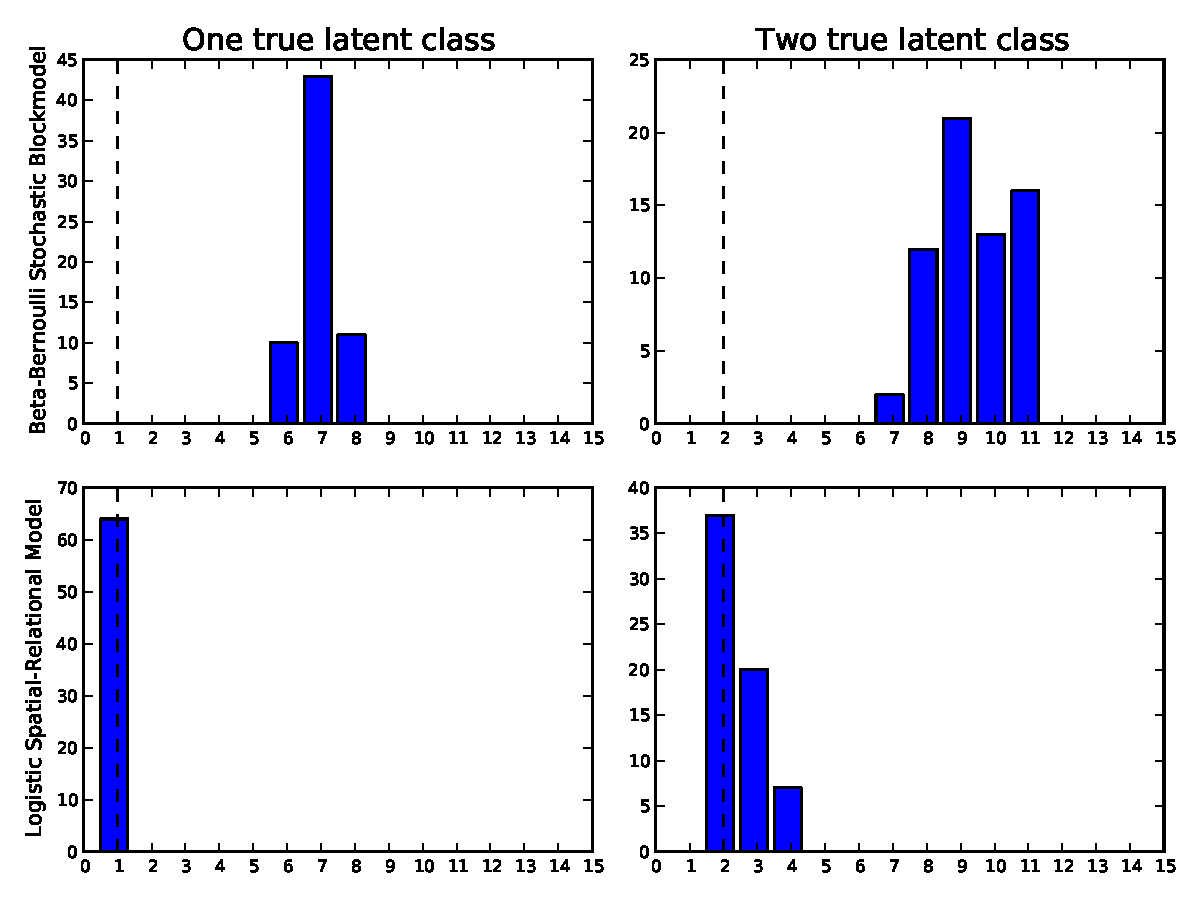
\includegraphics{comparison.ai}}
  \caption{\textbf{Visualizing type inference uncertainty.} Our fully
    Bayesian model gives a confidence estimate (posterior probability)
    that any two given cells are of the same type. In a.) we visualize
    that cell-cell coassignment matrix, showing the probability that
    cell i is of the same type as cell j on a range from 0.0 to
    1.0. The block structure shows subsets of cells which are believed
    to all belong to the same type. For comparison, b.) shows the
    anatomist-defined type for each cell, grouped broadly into the
    coarse types identified in the previous figure. c.) for each cell
    in the matrix, c.) shows the soma depth as well as the depth
    histogram for all putative synaptic contacts. \textbf{Link vs
      cluster accuracy} d.) The posterior distribution of ROC curves
    from 10-fold cross validation when predicting connectivity, as
    well as e.) the area under the curve and f.) the type agreements
    with known neuroanatomist types. g. A comparison of the predictive
    accuracy (area under the curve) for hand-labeled anatomical data,
    versus inclusion of additional sources of information, as well as
    the clustering accuracy. Note that our model sacrifices very
    little predictive accuracy for additional clustering accuracy. By
    comparison, conventional methods fail at one or both.  d. ) The
    spatial extent (in depth and area) of the types identified by
    humans and our various algorithmic approaches.}
\label{fig:mouseretina_compare}
\end{figure}

% from experiments/mouseretina/spatial_var.txt

% Relational Model: mean = 14.586508 std=8.136334
% Spatial-Relational Model: mean = 34.540355 std=1.069483
% Truth (fine): mean = 34.348443 std=7.567564
% Truth (coarse): mean = 35.276636 std=2.372951

\subsection*{Recovering spatial connectivity in multiple graphs simultaneously}

Having shown our model to work on the repeating tessellated, laminar
structure of the mammalian retina, we then apply our model to a
structurally very different connectome -- the whole body of a small
roundworm: \textit{Caenorhabditis elegans} is a model system in
developmental neuroscience\autocite{White1986}, with the location and
connectivity of each of 302 neurons developmentally determined,
leading to early measurement of the connectome. Unlike the retina,
only the motor neurons in C. elegans exhibit regular distribution in
space -- along the body axis. Most interneurons are concentrated in
various ganglia that project throughout the entire animal, and the
sensory neurons are primarily located in a small number of anterior
ganglia. \textit{C. elegans} also differs from the retina in that the
measured connectome is actually two separate graphs -- one of directed
chemical synapses and another of undirected electrical synapses. As
this is a very different connectome, it allows an interesting
generalization test: how well will our model work on such a distinct
data set.

\begin{figure}
  \centering 
  \centerline{\includegraphics[width=7.0in]{celegans2.ai}}
  \caption{Discovering connectivity and type in
    \textit{C. elegans}. a.) posterior distribution on cell
    connectivity as a function of discovered type, similar to
    figure~\ref{fig:mouseretina_compare}. In b.) we plot
    neuroanatomist-derived types along with their labels. Our model
    shows high probability of motor neurons, sensory neurons, and
    various interneuron classes being of the same type. Soma positions
    along the body axis are plotted in c.) where we see that we
    cluster spatially-distributed motor neurons together, whereas head
    sensory neurons are more likely to be grouped together as well.
    d.) The ROC curves for held-out link probability for both the
    electrical synapses (gap junctions) and chemical synapses in
    c. elegans. e.) The posterior distribution of the area under the
    ROC curve for the curves in d. f.) Measurements of the agreement
    of our identified cell types compared to neuroanatomists. The high
    compleneness but low homogeneity (and corresponding low ARI)
    reflects our model's tendency to group multiple types into a
    single type.}
  \label{fig:celegans}
\end{figure}



Using both the chemical and electrical connectivity (see methods), we
determined the underlying cell types explained by connectivity and
distance (fig~\ref{fig:celegans}a). A superficial inspection of the
results shows clustering into groups consisting roughly homogeneously
of motor neurons, sensory neurons, and interneurons. Closer
examination reveals agreement with the classifications originally
outlined by White in 1986.

Note our clustering does not perfectly reflect known divisions --
several combinations of head and sensory neurons are combined, and a
difficult-to-explain group of mostly VB and DB motor neuron types,
with VC split between various groups. Our identified cell types thus
reflect a ``coarsening'' of known types, based entirely on
connectivity and distance information, even when the organism exhibits
substantially less spatial regularity than the retina.

\subsection*{Types and connectivity in artificial structures}
\begin{figure}
  \centering 
  \centerline{\includegraphics[width=6in]{mos6502.ai}}
  \caption{Discovering connectivity and type the 6502 microprocessor.
    a.) is the micrograph of the original microprocessor, with the
    region containing the registers under study highlighted. b.) Our
    graph consists of the interconnections of MOS field-effect
    transistors with three terminals, Gate, C1, and C2. Reconstruction
    technique did not permit resolution of C1 and C2 into source and
    drain. c.) The spatial distribution of the transistors in each
    cluster show a clear pattern d.) The clusters and connectivity
    versus distance for connections between Gate and C1, Gate and C2,
    and C1 and C2 terminals on a transistor. Purple and yellow types have a
    terminal pulled down to ground and mostly function as
    inverters. The blue types are clocked, stateful transistors, green
    control the ALU and orange control the special data bus (SDB).}
  \label{fig:mos6502}
\end{figure}


To show the applicability of our method to other connectome-style
datasets, we obtained the spatial location and interconnectivity of
the transistors in a classic microprocessor, the MOS Technology 6502
(used in the Apple II) \autocite{James2010}. Computer architects use
common patterns of transistors when designing circuits, with each
transistor having a ``type'' in the circuit. We identified a region of
the processor with complex but known structure containing the primary
8-bit registers X, Y, and S (fig~\ref{fig:mos6502}).

Our algorithm identifies areas of spatial homogeneity that mirror the
known structure in the underlying architectural circuit, segmenting
transistor types recognizable to computer architects. Using the
original schematics, we see that one identified type contains the
``clocked'' transistors, which retain digital state. Two other types
contain transistors with pins C1 or C2 connected to ground, mostly
serving as inverters.  An additional identified type controls the
behavior of the three registers of interest (X, Y, and S) with respect
to the SB data bus, either allowing them to latch or drive data from
the bus. The repeat patterns of spatial connectivity are visible in
figure~\ref{fig:mos6502}c, showing the man-made horizontal and
vertical layout of the same types of transistors.


\section*{Discussion}
We have presented a machine learning technique that allows cell types
and microcircuitry to be discovered from connectomics data.  We have
shown its applicability to regularly structured laminar neural
circuits like the retina, as well as a less structured whole neuronal
organism (\textit{C. elegans}) and a classical processor. When
compared to existing methods, we show how the incorporation of all of
this data yields results that combine both high link-prediction
accuracy and high agreement with human anatomists. We have found that
combining the available data types allows us to discover cell types
and microcircuitry that were known to exist in the systems based on
decades of previous research and allows good prediction of
connectivity.

For our probabilistic models, no known solution exists to
exactly find the most probable parsing of the neurons into cell-types
and connectivity patterns. We employ a collection of Markov-chain
Monte carlo techniques (see Methods) but while different
initializations converge to similar ultimate values, we can never
realistically obtain the global optimum. There are a broad range of
techniques that may offer good approximations to the global optimum
and future work could adapt them to
find more precise solutions to our problem.

For our probabilistic model, inference becomes slower as the amount of
data increases. Our algorithm required several hours for 1000
neurons. Scaling this class of probabilistic model is an active area
of research, and recent results in both variational methods
\autocite{Hoffman2013} and spectral learning \autocite{Anandkumar2012}
and future work could adapt them to find faster approximate solutions
to our problem.

Larger datasets will allow algorithms to distinguish more distinct
types and we expect closer agreement with existing anatomical
knowledge as more data become available.  Moreover, in general, for
such problems precision increases with the size of the dataset and the
cells that we have are not sufficient to statistically distinguish all
the cell types known in anatomy (such as the $\sim 70$ in the
retina). Still, using only connectivity and distance it is possible to
meaningfully divide neurons into types.

Our small collection of hand-selected distance-dependent likelihood
functions are clearly non-exhaustive, and assume monotonicity
of connectivity probability -- for a given class, closer cells
are never less-likely to connect. This is known to be insufficient
for various neural systems. Future models could incorporate
a wider variety of likelihood functions, or even learn the global
functional form from the data. 

There exist a range of previous approaches to the discovery of neural
microcircuitry\autocite{Mountcastle1957, Douglas1991, Bartho2004,
  Freund1998}.  These generally involve a great deal of manual labor
and ad-hoc determination of what constitutes a “type” of cell -- to
this day there are disagreements in the literature as to the “true”
types in the mammalian retina. Much as phylogenomics has changed our
understanding of animal ontologies, modern large scale data will allow
the efficient unbiased discovery of cell types and circuits. The sheer
amount of available data demands the introduction of algorithmic
approaches.

The development of automatic identification and quantification of cell
type may also provide a new computational phenotype for quantifying
the effect of disease, genetic interventions, and
developmentally-experienced neural activity. Our method can in
principle identify neuron-types across non-connected graphs,
e.g. across animals. For example, the types of neurons in one animal
can be associated with the types of neurons in another animal, in the
same way as this is already possible through molecular marker
\autocite{Brown2009}. This could be particularly important if cell
types appear that are due to properties of the stimuli and experience
as opposed to just the molecular properties of cells, such as color
and orientation selective types in primary visual cortex
\autocite{Sincich2005,Lennie2005}. This would allow comparative
quantitative anatomy across animals, and aid the search for the
ultimate causes of connectivity.

Our model combines connectivity, cellular, and synaptic properties,
and suggests the way towards combining even richer data. Distinct cell
types differ in morphology, connectivity, transcriptomics, relation to
behavior or stimuli and many other ways. Algorithms combining this
data and type type information may allow us to synthesize all the
available information from one experiment or even across experiments
into a joint model of brain structure and function.

Our work shows how rich probabilistic models can contribute to computational neuroanatomy. 
Eventually, algorithms will have to become a central tool for
anatomists, as it will progressively become impossible for humans to
parse the huge datasets. This transition may follow a similar
transition to that of molecular biology (with gene-finding
algorithms) and evolutionary biology with (computational
phylogenetics). Ultimately, computational approaches may help resolve the significant
disagreements across human anatomists. 


\subsection*{Methods Summary}

For the basic link-distance model, we take as input a connectivity
matrix $R$ defining the connections between cell $e_i$ and $e_j$, as
well as a distance function $d(e_i, e_j)$ representing a (physical)
distance between adjacent cells.  See
the supplemental material for extension to multiple connectivity
matrices. We assume there exist an unknown number $K$ of latent
(unobserved) cell types, $k \in \{1, 2, 3, \dots, K\}$, and that each
cell $e_i$ belongs to a single cell type. We indicate a cell $e_i$ is
of type $k$ using the assignment vector $\vec(c)$, so $c_i = k$. The
observed connectivity between two cells $R(e_i, e_j)$ then depends
only on their latent type and their distance through a link function
$f(\cdot, d(e_i, e_j))$. We assume $f$ is parameterized based on the
latent type, $c_i=m$ and $c_j=n$, via a parameter$\eta_{mn}$, as well
as a set of global hyper parameters $\theta$, such that the link
function is $f(d(e_i, e_j) | \eta_{mn}, \theta)$.

We then jointly infer the maximum a posteriori (MAP) estimate of the
class assignment vector $\vec(c) = \{c_i\}$, the parameter matrix
$\eta_{mn}$, and the global model hyperparameters $\theta$ :

\begin{equation}
  p(\vec{c}, \eta, \theta | R ) \propto \prod_{i, j} p(R(e_i, e_j) | f(d(e_i, e_j) | \eta_{c_ic_j}), \theta) \prod_{m, n} p(\eta_{mn} | \theta)  p(\theta) p(\vec{c} | \alpha) p(\alpha) p(\theta)
\end{equation}

For the retina data, we then extend the model with the additional
features indicated. Cell soma depth is modeled as a
cell-type-dependent Gaussian with latent (unknown) per-type mean and
variance. Similarly, each cell has some number $N_i$ of synapses, 
each of which is drawn from a cell-type-specific density profile
with up to three modes.


Inference is performed in three steps via composable transition 
kernels -- one for structural, one for per-type parameters, and
one kernel for global parameters and hyperparameters. Details
of data preprocessing, inference parameters, and runtime can
be found in the Supplementary Methods section. 

\printbibliography

\begin{itemize}

 \item \textbf{Acknowledgments} We thank Josh Vogelstein for discussions and reading of the manuscript, Finale Doshi-Velez for early discussions on the model, and Erica Peterson, and Jonathan Glidden, and Yarden Katz for extensive manuscript review. Funding for compute time was provided by Amazon Web Services ``AWS in Education'' grants. 
\item \textbf{Author Contributions} KK and EJ developed model. EJ derived inference, implemented code, tested, and ran experiments. KK and EJ wrote manuscript text and solicited feedback. 
 \item \textbf{Competing Interests} The authors declare that they have no
competing financial interests.
 \item \textbf{Correspondence} Correspondence and requests for materials
should be addressed to E.J.~(email: jonas@eecs.berkeley.edu).
\end{itemize}

\newpage
\section*{Supplementary Methods }

\subsection*{Probabilistic Model}

Our model is a extension of the iSBM
\autocite{Kemp2006a,Xu2006} to incorporate spatial relations between entities,
inspired by attempts to extend these models with arbitrary
discriminative functions\autocite{Murphy2012}.

We take as input a connectivity matrix $R$ defining the connections
between cell $e_i$ and $e_j$, as well as a distance function $d(e_i,
e_j)$ representing a (physical) distance between adjacent cells. See
the supplemental material for extension to multiple connectivity
matrices. We assume there exist an unknown number $K$ of latent
(unobserved) cell types, $k \in \{1, 2, 3, \dots, K\}$, and that each
cell $e_i$ belongs to a single cell type. We indicate a cell $e_i$ is
of type $k$ using the assignment vector $\vec(c)$, so $c_i = k$. The
observed connectivity between two cells $R(e_i, e_j)$ then depends
only on their latent type and their distance through a link function
$f(\cdot, d(e_i, e_j))$. We assume $f$ is parameterized based on the
latent type, $c_i=m$ and $c_j=n$, via a parameter$\eta_{mn}$, as well
as a set of global hyper parameters $\theta$, such that the link
function is $f(d(e_i, e_j) | \eta_{mn}, \theta)$. 


We then jointly infer the maximum a posteriori (MAP) estimate of the
class assignment vector $\vec(c) = \{c_i\}$, the parameter matrix $\eta_{mn}$, and
the global model hyperparameters $\theta$ :

\begin{equation}
  p(\vec{c}, \eta, \theta | R ) \propto \prod_{i, j} p(R(e_i, e_j) | f(d(e_i, e_j) | \eta_{c_ic_j}), \theta) \prod_{m, n} p(\eta_{mn} | \theta)  p(\theta) p(\vec{c} | \alpha) p(\alpha) p(\theta)
\end{equation}


% Methods section 3000 words
% methods summary does not appear in the online text
% methods section can have no figures or tables [grrr]



We describe the spatial ``Logistic-distance Bernoulli''  function here,
and others in the supplemental material. 

% fixme class component, NOT class
The ``logistic-distance Bernoulli'' spatial model assumes that, if cell
$e_i$ is of type $m$ and cell $e_j$ is of type $n$, then $\eta_{mn}
= (\mu_{mn}, \lambda_{mn})$, and the probability that two cells $e_i$
and $e_j$ are connected is given by
\begin{eqnarray}
p^* &=& \frac{1.0}{1 + \exp \frac{d(e_i, e_j) - \mu_{mn}}{\lambda_{mn}}}\\
p &= & p^* \cdot (p_{max} - p_{min}) + p_{min}
\end{eqnarray}
where $p_{max}$ and $p_{min}$ are global per-graph parameters. 

We place an exponential priors on the latent parameters:
\begin{eqnarray}
 \mu_{mn} \sim \exp(\mu | \mu^{hp}) \\
\lambda_{mn} \sim \exp(\lambda | \lambda^{hp})
\end{eqnarray}

using  $\lambda^{hp}$ and $\mu^{hp}$ as global per-graph hyperparameters. 

We use a Dirichlet-process prior on class assignments, which allows
the number of classs to be determined automatically. In brief, for $N$
total cells, the probability of a cell belonging to a class is
proportional to the number of datapoints already in that class, $N_k$,
such that $p(c_i = k) \propto \frac{m_k}{N + \alpha}$ and the
probability of the cell belonging to a new class $k'$ is $p(c_i = k')
\propto \frac{\alpha}{N + \alpha}$. $\alpha$ is the global
concentration parameter -- larger values of $\alpha$ make the model
more likely to propose new classes. We grid the parameter $\alpha$ and
allow the best value to be learned from the data.


Where we model cell depth, we assume that 
each cell type has a typical depth, and thus a Gaussian distribution
of $s_i$. We assume $s_i \sim N(\mu^{(s)}_k,
\sigma^{2(s)}_k)$, where the $(s)$ superscript indicates
these model parameters are associated with the soma-depth 
portion of our model.  We use a conjugate prior for $(\mu^{(s)}_k, \sigma^{2(s)}_k)$ with
$\mu^{(s)}_k \sim N(\mu^{(s)}_{hp}, \sigma^{2(s)}_k/ \kappa^{(s)}_{hp})$ and $\sigma^{2(s)}_k \sim
\chi^{-1}(\sigma^{2(s)}_{hp}, \nu^{(s)}_{hp}$. The use of conjugacy simplifies inference while allowing for each cell-type to have its own depth mean and distribution. 

Where we model synapse depth profile, we assume that each cell
type has a characteristic depth distribution of synaptic contact points, and thus
a mixture of Gaussians distribution over cell $i$’s $N_i$ contact points, $\vec{g^i}$.
We do this by assuming the $g^i_j$
are drawn from an $M=3$-component mixture of Gaussians. Thus associated with each cell type $k$ is a vector
of $M$ Gaussian means $(\mu^g_{k,1}, \cdots, \mu^g_{k, M})$, and a
mixture vector $\pi_k$.  This representation can thus model depth distributions of contact points that have up to three modes, an assumption that is well matched in the bulk of anatomical studies of cell-type dependent connectivity.


\subsection*{Inference} 
We perform posterior inference via Markov-chain Monte Carlo (MCMC),
annealing on the global likelihood during the traditional burn-in
phase. MCMC transition kernels for different parts of the state space
can be chained together to construct a kernel whose ergodic
distribution is the target ergodic distribution over the entire state space. 

Our first transition kernel (``structural'') performs gibbs sampling 
of the assignment vector $p(\vec{c} | \eta, \theta, \alpha)$. 
The lack of conjugacy in our likelihood model makes an explicit 
evaluation of the conditional assignment probabilities impossible, 
motivating us to use an auxiliary variable method \autocite{Neal2000}
in which a collection of ephemeral classs are explicitly represented
for the duration of the Gibbs scan. 

We then employ a transition kernel to update the per-component
parameter values $\eta_{mn}$. Conditioned on the assignment vector
$\vec{c}$ and the model hyperparameters $\theta, \alpha$ the 
individual $\eta_{mn}$ are independent. We slice sample \autocite{Neal2003}
each component's parameters, choosing the slice width as a function
of the global hyperparameter range. 

The global hyper-parameters, both $\alpha$ and $\theta$, are allowed
to take on a discrete set of possible values. As $\theta$ is often a
tuple of possible values, we explore the cartesian product of all
possible values. We then Gibbs sample (our final transition kernel),
which is always possible in a small, finite, discrete state space.

We chain these three kernels together, and then globally anneal on the
likelihood from a temperature of $T=64$ down to $T=1$ over $900$
iterations unless otherwise indicated, and then run the chain for
another $100$ iterations. We then generate at least $20$ samples, each
taken from the end of a single Markov chain initialized from different
random initial points in the state space. For visualization we pick the
chain with the highest log likelihood, but for all numerical
comparisons (including link probability and cluster accuracy) we use this full
collection of samples from the posterior distribution to estimate the
resulting statistics.

\subsection*{Link Prediction}
As a proxy for link-prediction accuracy we compute the probability of a link
between two cells using each model, trained fully on the data. While this method
is potentially prone to overfitting, the overfitting will be shared across models
and in fact will preferentially bias in favor of competing models
which over-cluster the data. We use a full collection of posterior samples when
computing the link probability, and then compute the area under the ROC curve for
each. 

\subsection*{Model Comparison}
We compare our model with a standard network clustering model, the
latent-position clustering model. This model assumes each cell belongs
to one of K clusters, and each cluster is associated with a
$d-$dimensional Gaussian distribution. The probability of a link is
then a function of the distance between the data points in this
continuous-space. We use \autocite{Salter-Townshend2013} a variational
implementation provided in R, parametrically varying the number of
latent dimensions and the number of requested groups.  While this
model provides reasonable link predictive accuracy, the clusterings
dramatically disagree with those from human anatomists.


\subsection*{Parameters}

Hierarchical generative models can be sensitive to hyperparameter
settings, thus for most hyperparamters we perform inference. In cases
where we cannot we run separate collections of markov chains at
separate settings and show the results across all pooled
parameters. For the case of the mouse retina data, we consisder
maximum link probability $p_{max} \in \{0.95, 0.9, 0.7\}$, variance
scales for the synapse density profile of $\sigma^2 \in \{0.01, 0.1,
1.0\}$ (of normalized depth), and $K \in \{2, 3\}$ possible synapse
density profile mixture components. For the connectivity-distance-only
model we actually perform inference over both $p_{max}$ and $p_{min}$.


\subsubsection*{Mixing of our Markov chains} 
Evaluating whether or not approximate inference methods, such as MCMC,
produce samples which are valid approximations of the posterior
distribution is an ongoing area of research in the computational
statistics community. We use a rough proxy here -- synthetic
likelihood evaluation.  For synthetic datasets of sizes comparable to
our real data size, do we recover known ground truth information after
running our markov chains for the appropriate amount of time?

Figures \ref{fig:mixing:ari} and \ref{fig:mixing:scorevstime} shows
the cluster accuracy (ARI) to ground truth and the total log score as a function of
runtime.  We see dramatic changes in log score initially as we vary
the temperature, stabilizing as runtime progresses, for each
chain. Then we see the characteristic jumps between nearby modes
towards the end of the run, in both log score and ARI.  Importantly,
regardless of whether our model over- or under-estimates the exact
posterior variance about the network, we find points in the latent
variable space that are both predictive \textit{and} parsimonious,
largely agreeing with the human anatomists and predicting existing
connections.

\begin{figure}
  \centering 
  \centerline{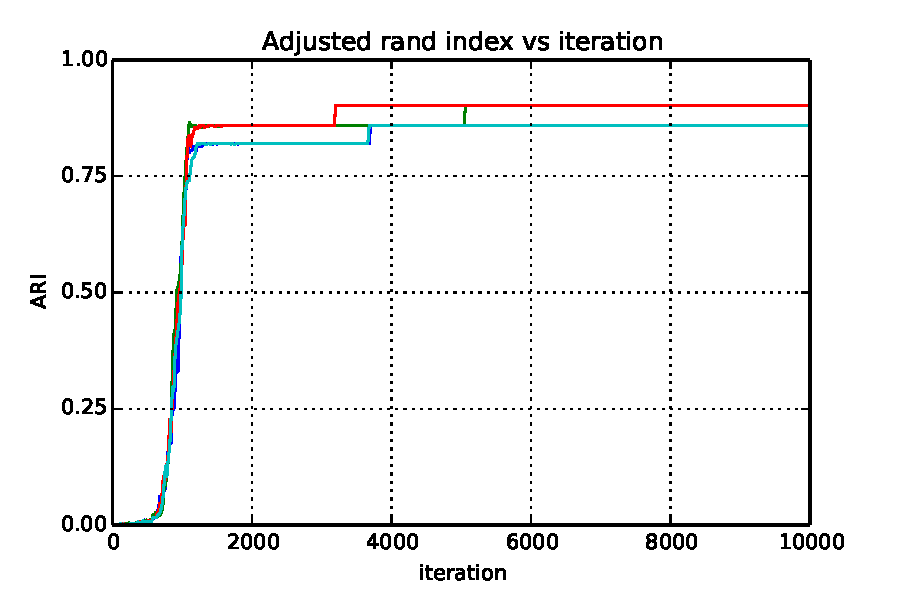
\includegraphics[width=60mm]{mixing.ari.pdf}}
  \caption{Adjusted rand index for synthetic data as a function of run iteration. }
\label{fig:mixing:ari}
\end{figure}

\begin{figure}
  \centering 
  \centerline{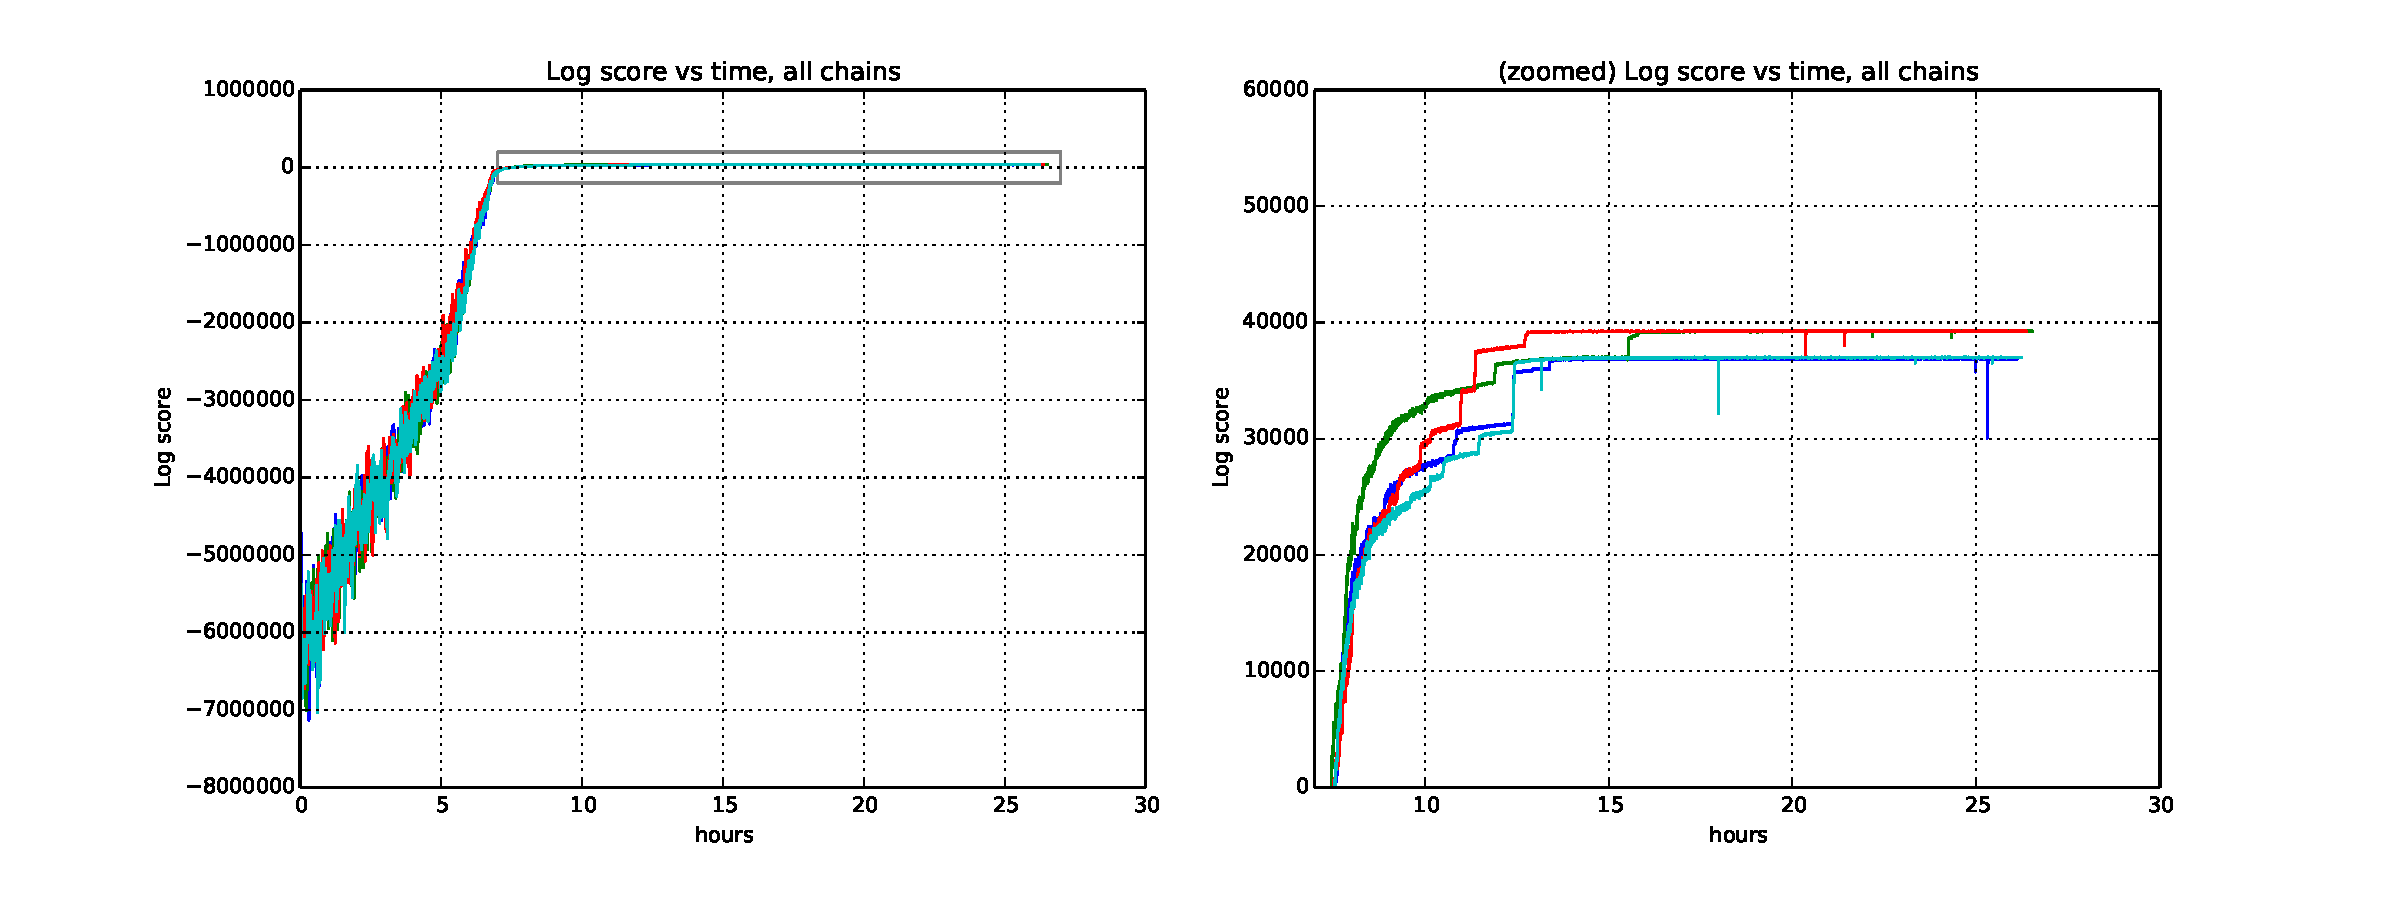
\includegraphics[width=130mm]{mixing.scorevstime.pdf}}
  \caption{Total model score (log score) vs iteration}
\label{fig:mixing:scorevstime}
\end{figure}


\subsection* {Mouse Retina}
\label{supp:mouseretina}
Dense serial electron microscopy of a $114\mu m \times 80 \mu m $ area
in the mouse retina by \autocite{Helmstaedter2013} yielded a listing
of places where neurons come into contact. There were over 1000 cells
originally, and selected the $950$ for which the location of the soma
could be reconstructed from the provided cell plots (soma locations
were not provided by the study's authors in machine-readable
form). Ultimately this left a matrix between the total synapse-like
contact area between all pairs of 950 cells. Area was thresholded at
$0.1\mu m$, determined by hand, to yield a 950 $\times$ 950 entry
matrix that served as input to our algorithm. We measured the distance
between cells using the reconstructed soma centers, and used the
Logistic-Distance spatial relation. Hyperprior griddings are shown in
supplemental section \ref{supp:hyperpriors}.

\subsection*{C. elegans}

We obtained the connectome of c. elegans from data published
previously \autocite{Varshney2011}, and isolated the 279 nonpharyngeal
neurons, with a total of 6393 chemical synapses and 890 gap junctions
originally cleaned up in \autocite{Chen2006}. A cell's position was
its distance along the anterior-posterior axis normalized between zero
and one. We used both networks, the chemical network as a directed
graph and the electrical network as undirected graph. We use the
synapse counts with the logistic-distance poisson likelihood, scaling
the counts by 4.0 to compensate for the Poisson's overdispersion.


\subsection*{Microprocessor}
We extracted the connection graph for the transistors in the MOS6502
\autocite{visual6502source}. Each transistor has three terminals (gate,
source, drain), but the methods of the original dataset were unable to
consistently resolve which of the C1 and C2 terminals were source and
drain, leading to ambiguity in our encoding. We identified a region
consisting of three registers X, Y, and S via visual
inspection and focused our efforts there. We created a total of six
connectivity matrices by examining possible terminal pairings. One
graph, for example, $R^{gc_1}(e_i, e_j)=1$ if transistor $e_j$ and
$e_j$ are connected via pins $g$ and $c_1$. 


% \begin{addendum}
%  \item Put acknowledgements here.
%  \item[Competing Interests] The authors declare that they have no
% competing financial interests.
%  \item[Correspondence] Correspondence and requests for materials
% should be addressed to A.B.C.~(email: myaddress@nowhere.edu).
% \end{addendum}
\newpage
\section*{Supplemental Material}

\subsection*{Other Likelihoods}
\label{supp:otherlikelihoods}

We reparameterized the Logistic-Distance Bernoulli likelihood to
better capture the microprocessor data structure. We are explicitly
setting the maximum probability $p$ of the logistic function on a
per-component basis, drawing from a global $p \sim \operatorname{Beta}(\alpha_{hp},
\beta_{hp})$. Then $\lambda$ is set for each component as a global
hyperparameter, $\lambda$.

The ``logstic-distance Poisson'' spatial model is used to explicitly
mode the count of synapses, $c$, between two neurons. The probability
of c synapses between two neurons is distributed $c \sim
\textrm{Poisson}(c | r)$, where $r$ (the ``rate'') is generated by a
scaled logistic function (the logistic function has range $[0,
1]$. For each component $\eta_{mn}$ we learn both the threshold
$\mu_{mn}$ and the rate scaling factor $r_{mn}$ Thus if for cells $m$
and $n$ are likely to have on average $20$ synases if they are closer
than $5 \mu m$, then $\mu_{mn} = 5$ and $r_{mn} = 20$ "

Thus the probability of $R(e_i, e_j) = c$ synapses between two cells $e_i$ and $e_j$ is given by:
\begin{eqnarray}
r^* &=& \frac{1.0}{1 + \exp \frac{d(e_i, e_j) - \mu_{mn}}{\lambda}}\\
r & = & r^* \cdot (r_{mn} - r_{min}) + r_{min} \\
R(e_i, e_j) \sim \textrm{Poisson}(c | r)
\end{eqnarray}

where $\lambda$ and $r_{min}$ are per-graph parameters. Per-component parameters $\mu_{mn} \sim \exp(\mu | \mu^{hp})$ and $r_{mn} \sim \exp(r_{mn} | r_{scale}^{hp})$. 

\subsection*{Source code and data}

All source code and materials for running experiments can be
obtained from the project website, at \\

\href{http://https://github.com/ericmjonas/netmotifs}{https://github.com/ericmjonas/netmotifs/}

and the content of this paper along with scripts to run
experiments and generate all figures can be found at

\href{http://https://github.com/ericmjonas/netmotifs}{https://github.com/ericmjonas/connect-disco-paper/}

All preprocessed data has been made publicaly available as well. 

Please contact the author for pre-publication access. 

\subsection*{Extension to multiple graphs}
\label{supp:multigraph}
The model can handle multiple graphs $R^q$ simultaneously with a shared clustering by extending the likelihood to include the product of the likelihoods of the individual graphs. 

\begin{equation}
  p(\vec{c}, \{\eta^q\}, \{\theta^q\} | \{R^q\} ) \propto \prod_q \Bigg(\prod_{i, j} p(R^q(e_i, e_j) | f(d(e_i, e_j) | \eta^q_{c_ic_j}, \theta^q) \prod_{m, n} p(\eta^q_{mn} | \theta^q)  p(\theta^q) \Bigg) p(\vec{c} | \alpha) p(\alpha) 
\end{equation}

\FloatBarrier
\subsection*{Hyperprior grids and hyperprior inference}
\label{supp:hyperpriors}

For the mouse retina Logistic-Distance Bernoulli model, we gridded
$\mu^{hp}$ and $\lambda^{hp}$ into 40 $\log_{10}$-spaced points 1.0
and 80. 

For the c. elegans data with the Logistic Distance poisson model, we
gridded $\mu_{hp}$ and $\lambda$ into 20 $\log_{10}$-spaced points
bween 0.2 and 2.0, and the $ratescale^{hp}$ parameter into 20
$\log_{10}$-spaced points between 2.0 and 20.0. We globally set
$rate_{min}=0.01$.

For the microprocessor with the Logistic Distance fixed lambda
Bernoulli likelihood, we gridded $mu_{hp}$ into 50 $\log_{10}$-spaced
points between 10 and 500 and set $\lambda=\mu_{hp}/10$. $p_{min} \in
\{0.001, 0.01, 0.02\}$ and both $p_\alpha$ and $p_\beta \in \{0.1,
1.0, 2.0\}$.

\section*{Measuring clustering similarity}
We compare discovered types to known types via cluster comparison
metrics: cluster homogeneity, cluster completeness, and the adjusted
Rand index. Homogeneity measures how many true types are in a given
found type. If every cell type is split into two types, each subtype
is still completely homogeneous. Completeness measures how many
members of a given true type are split across found types.

The adjusted rand index (ARI) takes into account both effects
\autocite{Hubert1985} -- two identical clusterings have an ARI of 1.0
while progressively more dissimilar clusters have lower ARIs, becoming
slightly negative as the clustering gets anti-correlated.

Figure~\ref{fig:s:comparison} shows the result of taking 20 different clusters
and moving data points between them according to the following operations
\begin{itemize}
\item \textbf{distribute}: take a class and distribute its elements
  uniformly among the remaining types.
\item \textbf{merge} : take a type and merge it into another existing
  type
\item \textbf{split} : take a type and split it into two distinct
  types.
\end{itemize}

We can see the impact on ARI, completeness, and homogeneity as we
perform these operations on more of the original 20 types. In all
cases, ``distribution'' of one type among the others is detremental to
the metric. Splitting impacts completeness but not homogeneity, and
merging impacts homogeneity but not completness.



\begin{figure}
  \centering 
  \centerline{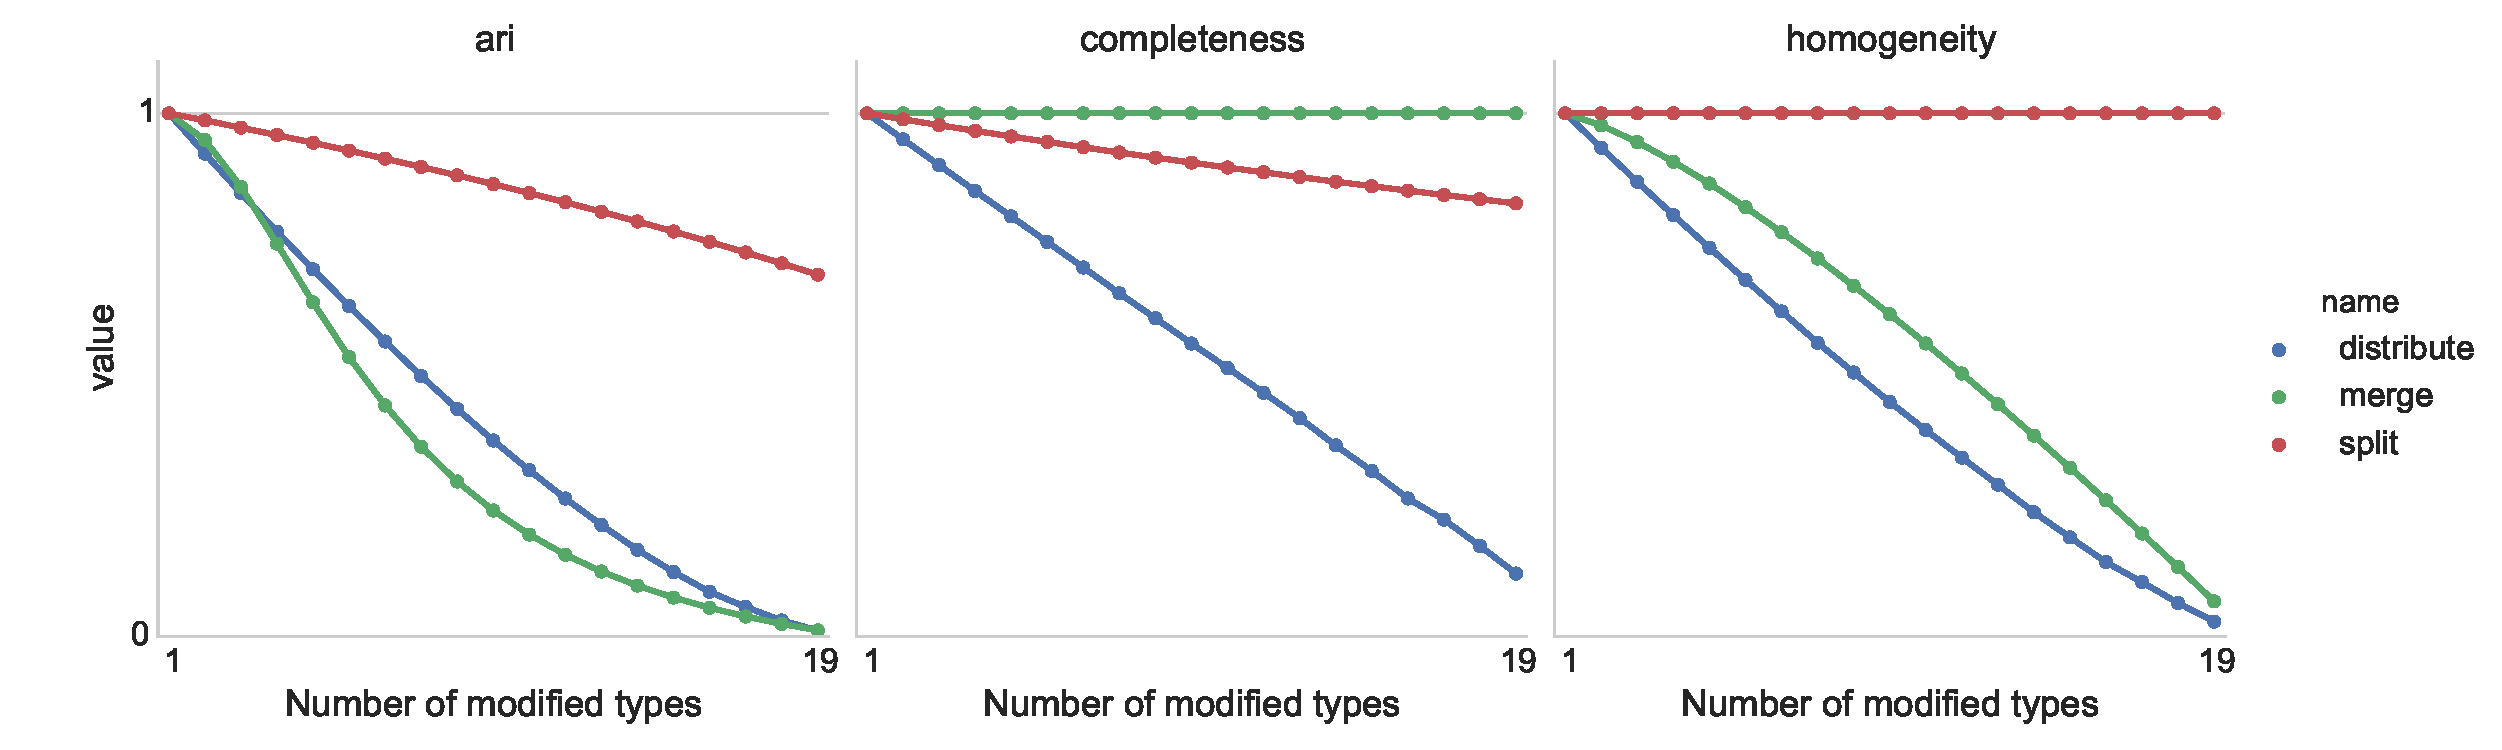
\includegraphics[width=180mm]{cluster_metric_comparison.pdf}}
  \caption{Type agreement evaluation metrics as a function of splitting types, merging types, and randomly distributing cells between types}
  \label{fig:s:comparison}
\end{figure}

\end{document}









